David Rohrbaugh

2014-10-31

Prototyping the Intake Mechanism and Joystick Control

\begin{tabular}{|p{5cm}|p{5cm}|}
 \hline
 This week I and several teammates worked on prototyping the intake mechanism.
 &
 Our current intake mechanism is a folded carboard panel. It will most likely be replaced by a more suitable material. This material must be able to deflect enough, however, to collect balls when the robot is up against a wall.
 \\
 \hline
\end{tabular}

\medskip

This is a diagram of our current prototype for the intake mechanism. A Tetrix channel is attached to a DC motor so it rotates as shown. The carboard, which will probably be replaced by a more suitable material, makes contact with both sizes of balls, pushing them into our yet-to-be-constructed launching mechanism.

\begin{center}
 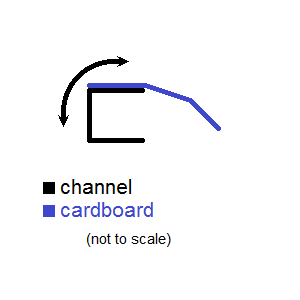
\includegraphics[width=215px]{./Entries/Images/intakePrototype.png}
\end{center}
